\documentclass[portrait,a0,final,19pt]{a0poster}
%%%Load packages
\usepackage{multicol} 			%2-column layout
% \setlength\columnsep{8pt} % This is the default columnsep for all pages
\usepackage[left=2cm,right=2cm,bottom=2cm,top=0cm]{geometry}			%Reset margins
\usepackage{helvet}				%Load Helvetica font & CM math
\usepackage{color}				%Needed for colour boxes & coloured text
% \usepackage{graphics}
\usepackage{graphicx}
\usepackage{subcaption}
\usepackage[font=Large,labelfont=bf]{caption}
\usepackage{float}
\usepackage{tikz}
\usetikzlibrary{arrows,positioning, shapes.symbols,shapes.callouts,patterns,shapes,chains,calc,backgrounds,fadings}

\usepackage{titlesec}
\usepackage{tabularx, booktabs} % make width of table columns evenly distributed (see http://tex.stackexchange.com/questions/60601/evenly-distributing-column-widths)

\usepackage{enumitem}
\usepackage{animate}[2017/05/18]

\usepackage{hyperref}
\usepackage{xcolor}

% \usepackage{titlepic}
% \usepackage{columns}

\titlespacing\section{0pt}{10pt plus 4pt minus 2pt}{5pt plus 2pt minus 2pt}
\titlespacing\subsection{0pt}{12pt plus 4pt minus 2pt}{0pt plus 2pt minus 2pt}

\titleformat*{\section}{\Huge\bfseries}
\titleformat*{\subsection}{\Large\bfseries}
\titleformat*{\subsubsection}{\large\bfseries}
\titleformat*{\paragraph}{\large\bfseries}
\titleformat*{\subparagraph}{\large\bfseries}

%%%Define colours and lengths
\definecolor{headingcol}{rgb}{0,0,0}			%Colour of main title
\definecolor{boxcol}{rgb}{0.7,0.2,0.2}		%Edge-colour of box and top banner
\fboxsep=1cm							%Padding between box and text
\setlength{\columnsep}{2cm}				%Set spacing between columns
\renewcommand{\familydefault}{\sfdefault}	%Set main text to sans-serif

%%%Format title
\makeatletter							%Needed to include code in main file
\renewcommand\@maketitle{%
\null									%Sets position marker
% \vspace{5em}
{
\color{headingcol}\sffamily\VeryHuge		%Set title font and colour
\@title \par}%
\vskip 0.6em%
{
\color{black}\sffamily\LARGE				%Set author font and colour
\lineskip .5em%
\begin{tabular}[t]{l}%
\@author
\end{tabular}\par}%
\vskip 1cm
\par
}
\makeatother



\title{Disease Knowledge Transfer across Neurodegenerative Diseases}

\newcommand{\inst}[1]{$^{#1}$}

\author{\Large{R\u{a}zvan V. Marinescu\inst{1}, Neil P. Oxtoby\inst{1}, Alexandra L. Young\inst{1}, Arman Eshaghi\inst{2}, Peter A. Wijeratne\inst{1}, Daniel C. Alexander\inst{1}}\\
\begin{tabular}{l p{1cm} l p{1cm} l}
\large{$^1$Centre for Medical Image Computing, University College London}  & & \large{$^2$Queen Square MS Centre, UCL Institute of Neurology} \\
\end{tabular}
}

% \author{R\u{a}zvan V. Marinescu\inst{1,2} \and Marco Lorenzi\inst{5} \and Stefano B. Blumberg\inst{1} \and Alexandra L. Young\inst{1} \and Pere Planell-Morell\inst{1} \and Neil P. Oxtoby\inst{1} \and Arman Eshaghi\inst{1,3} \and Keir X. Young\inst{4} \and Sebastian J. Crutch\inst{4} \and Polina Golland\inst{2} \and Daniel C. Alexander\inst{1}\\
% \begin{tabular}{l p{1cm} l p{1cm} l}
% \large{$^1$Centre for Medical Image Computing, University College London}  & & \large{$^2$Queen Square MS Centre, UCL Institute of Neurology} \\
% \end{tabular}
% } 



\begin{document}
% \hspace{-3cm}								%Align with edge of page, not margin
% \vspace{2cm}
% \includegraphics[scale=1,trim=0 0 0 200, clip]{Black_Landscape.pdf}

%\colorbox{boxcol}{							%Coloured banner across top
\begin{minipage}{50cm}					%Minipage for title contents
% \vspace{-18cm}
\maketitle
\end{minipage}
%}
% \vspace{-4cm}

\begin{multicols}{2}							
\raggedcolumns							%Don't stretch contents vertically

\pagenumbering{gobble}

%%%Column1
\vspace{-3em}
\section*{Introduction}



\begin{itemize}
 \item Recently disease progression models work well on large, multimodal datasets
 \item Datasets on rare neurodegenerative diseases (e.g., Posterior Cortical Atrophy) are limited and cross-sectional.
\end{itemize}

% \vspace{-0.5em}

\section*{Aim}

Develop a transfer learning model to transfer knowledge between diseases 



% \begin{figure}[H]
% 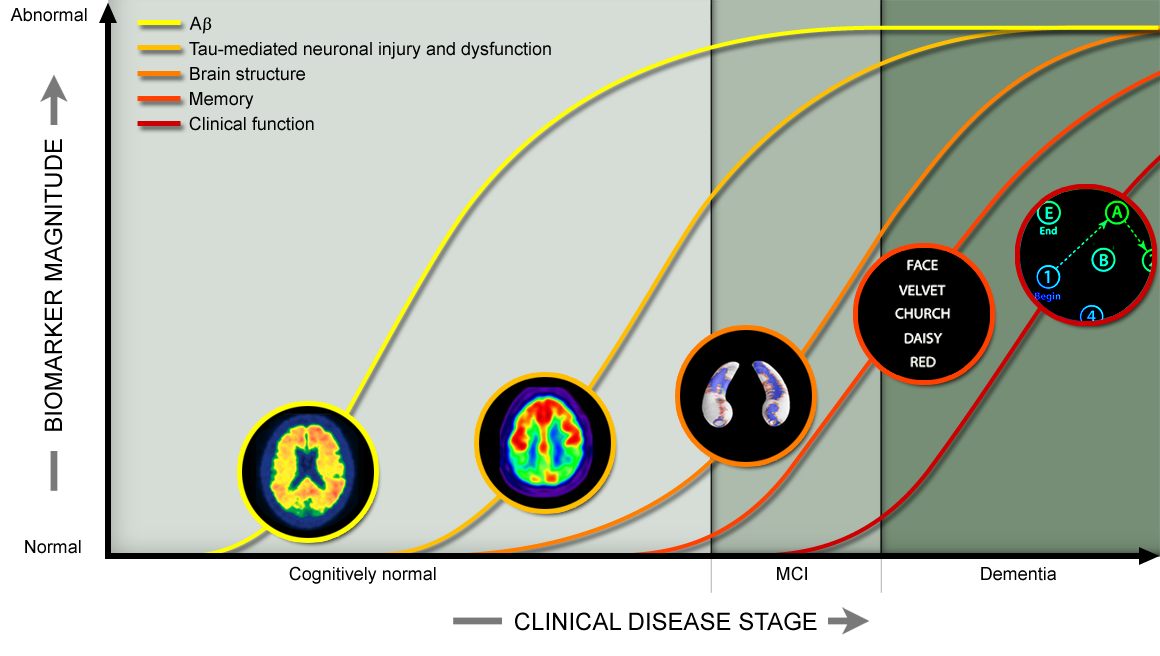
\includegraphics[width=0.31\textwidth,trim=0 50 0 0, clip]{adniDiseaseProgression}
% \caption{Hypothetical progression of typical Alzheimer's disease. The earliest biomarkers that become abnormal are the accumulation of abnormal amyloid-beta and tau proteins, which have a misfolded (i.e. abnormal) 3D structure. This is followed by structural integrity from MRI and finally cognitive decline as measured by cognitive tests.}
% \end{figure}




\section*{Method}



\begin{itemize}
 \item We propose Disease Knowledge Transfer:
 \begin{itemize}
   \item 
 \end{itemize}

\end{itemize}


% \subsection{Method Overview}

\newcommand{\lp}{\lambda_{d_i}^{\psi(k)}}
\newcommand{\lpuu}{\lambda_{d_i}^{\psi(k),(u)}}
\newcommand{\lpum}{\lambda_{d_i}^{\psi(k),(u-1)}}

\begin{equation}
\label{eqDysfunctionScoreDef}
 \gamma_{ij}^l = f(\beta_{i} + m_{ij}; \lambda_{d_i}^l)
\end{equation}


\begin{equation}
 p(y_{ijk}|\theta_k, \lp, \beta_{i}, \epsilon_k) = N(y_{ijk}| g( \gamma_{ij}^{\psi(k)} ; \theta_k), \epsilon_k)
\end{equation}


\begin{equation}
\label{eq:dktFinal}
 p(\boldsymbol{y}|\theta, \lambda, \beta , \epsilon) = \\ \prod_{(i,j,k) \in \Omega} p(y_{ijk}|\theta_k, \lp, \beta_{i}) 
\end{equation}


\begin{figure}[H]
 \centering
 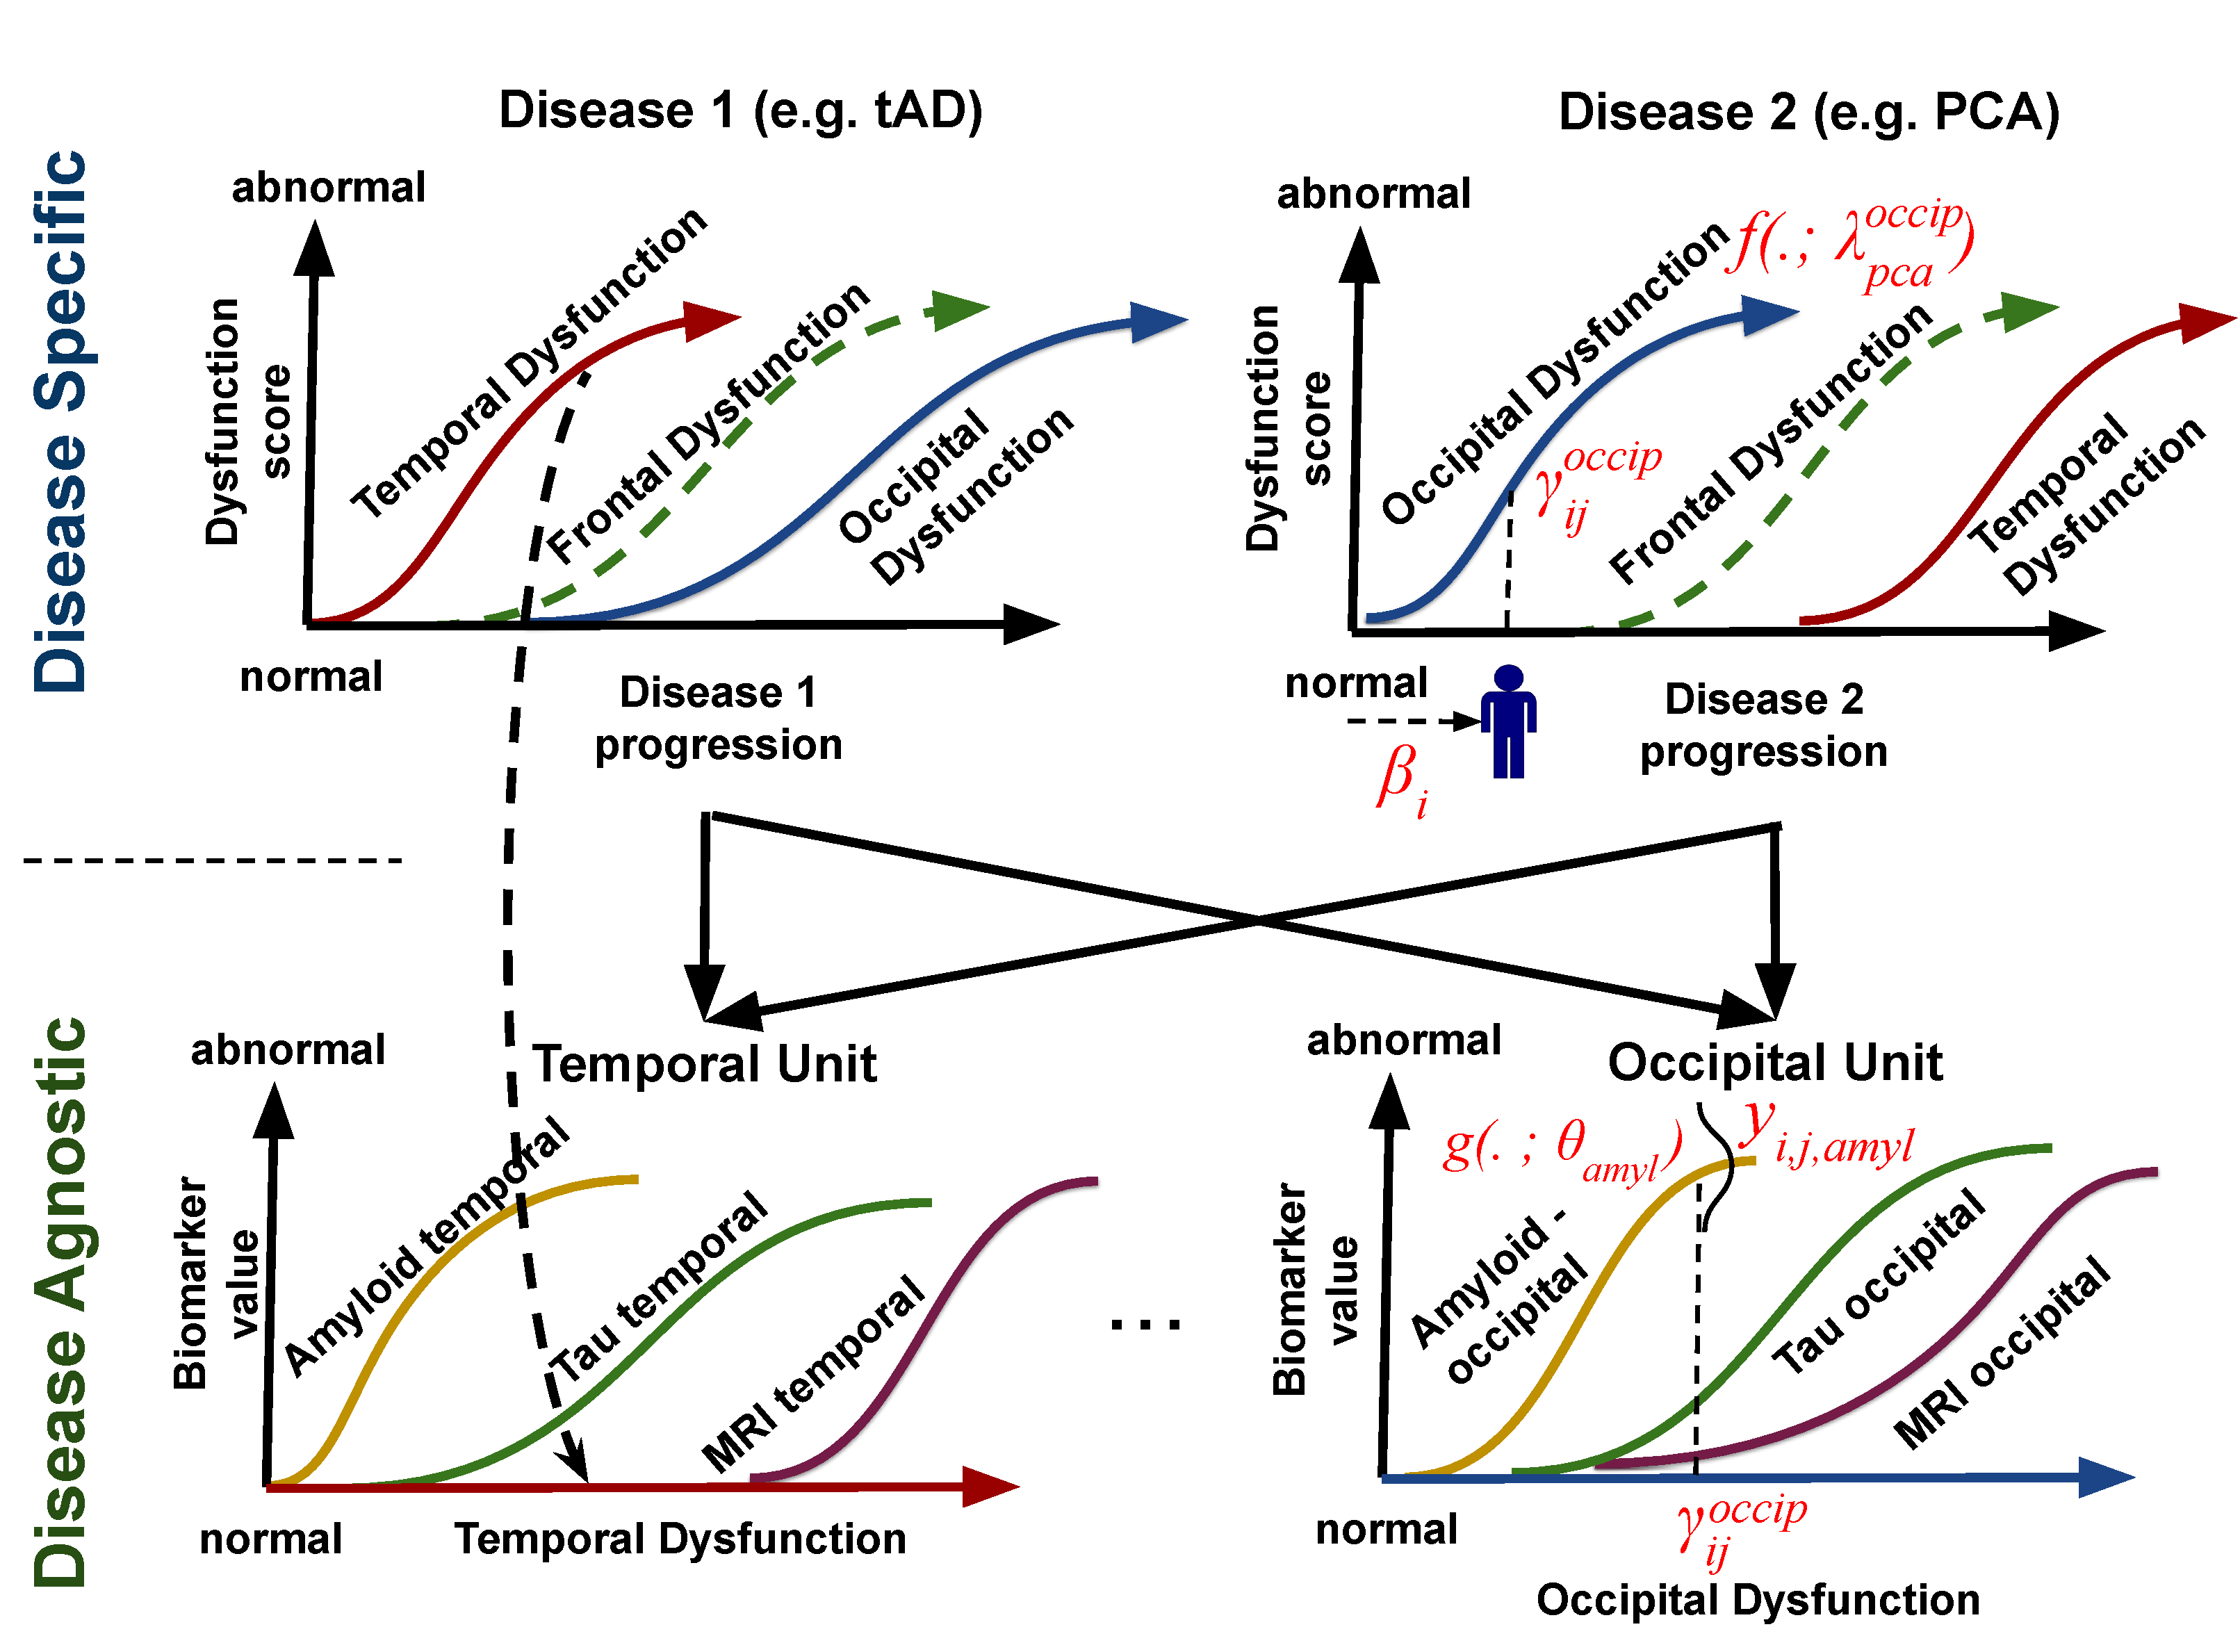
\includegraphics[width=0.4\textwidth,]{../figures/disease_knowledge_transfer_symbols.pdf}
 \caption{}
 \label{fig:diagram}
\end{figure}



\section*{Results}


\begin{figure}[H]
%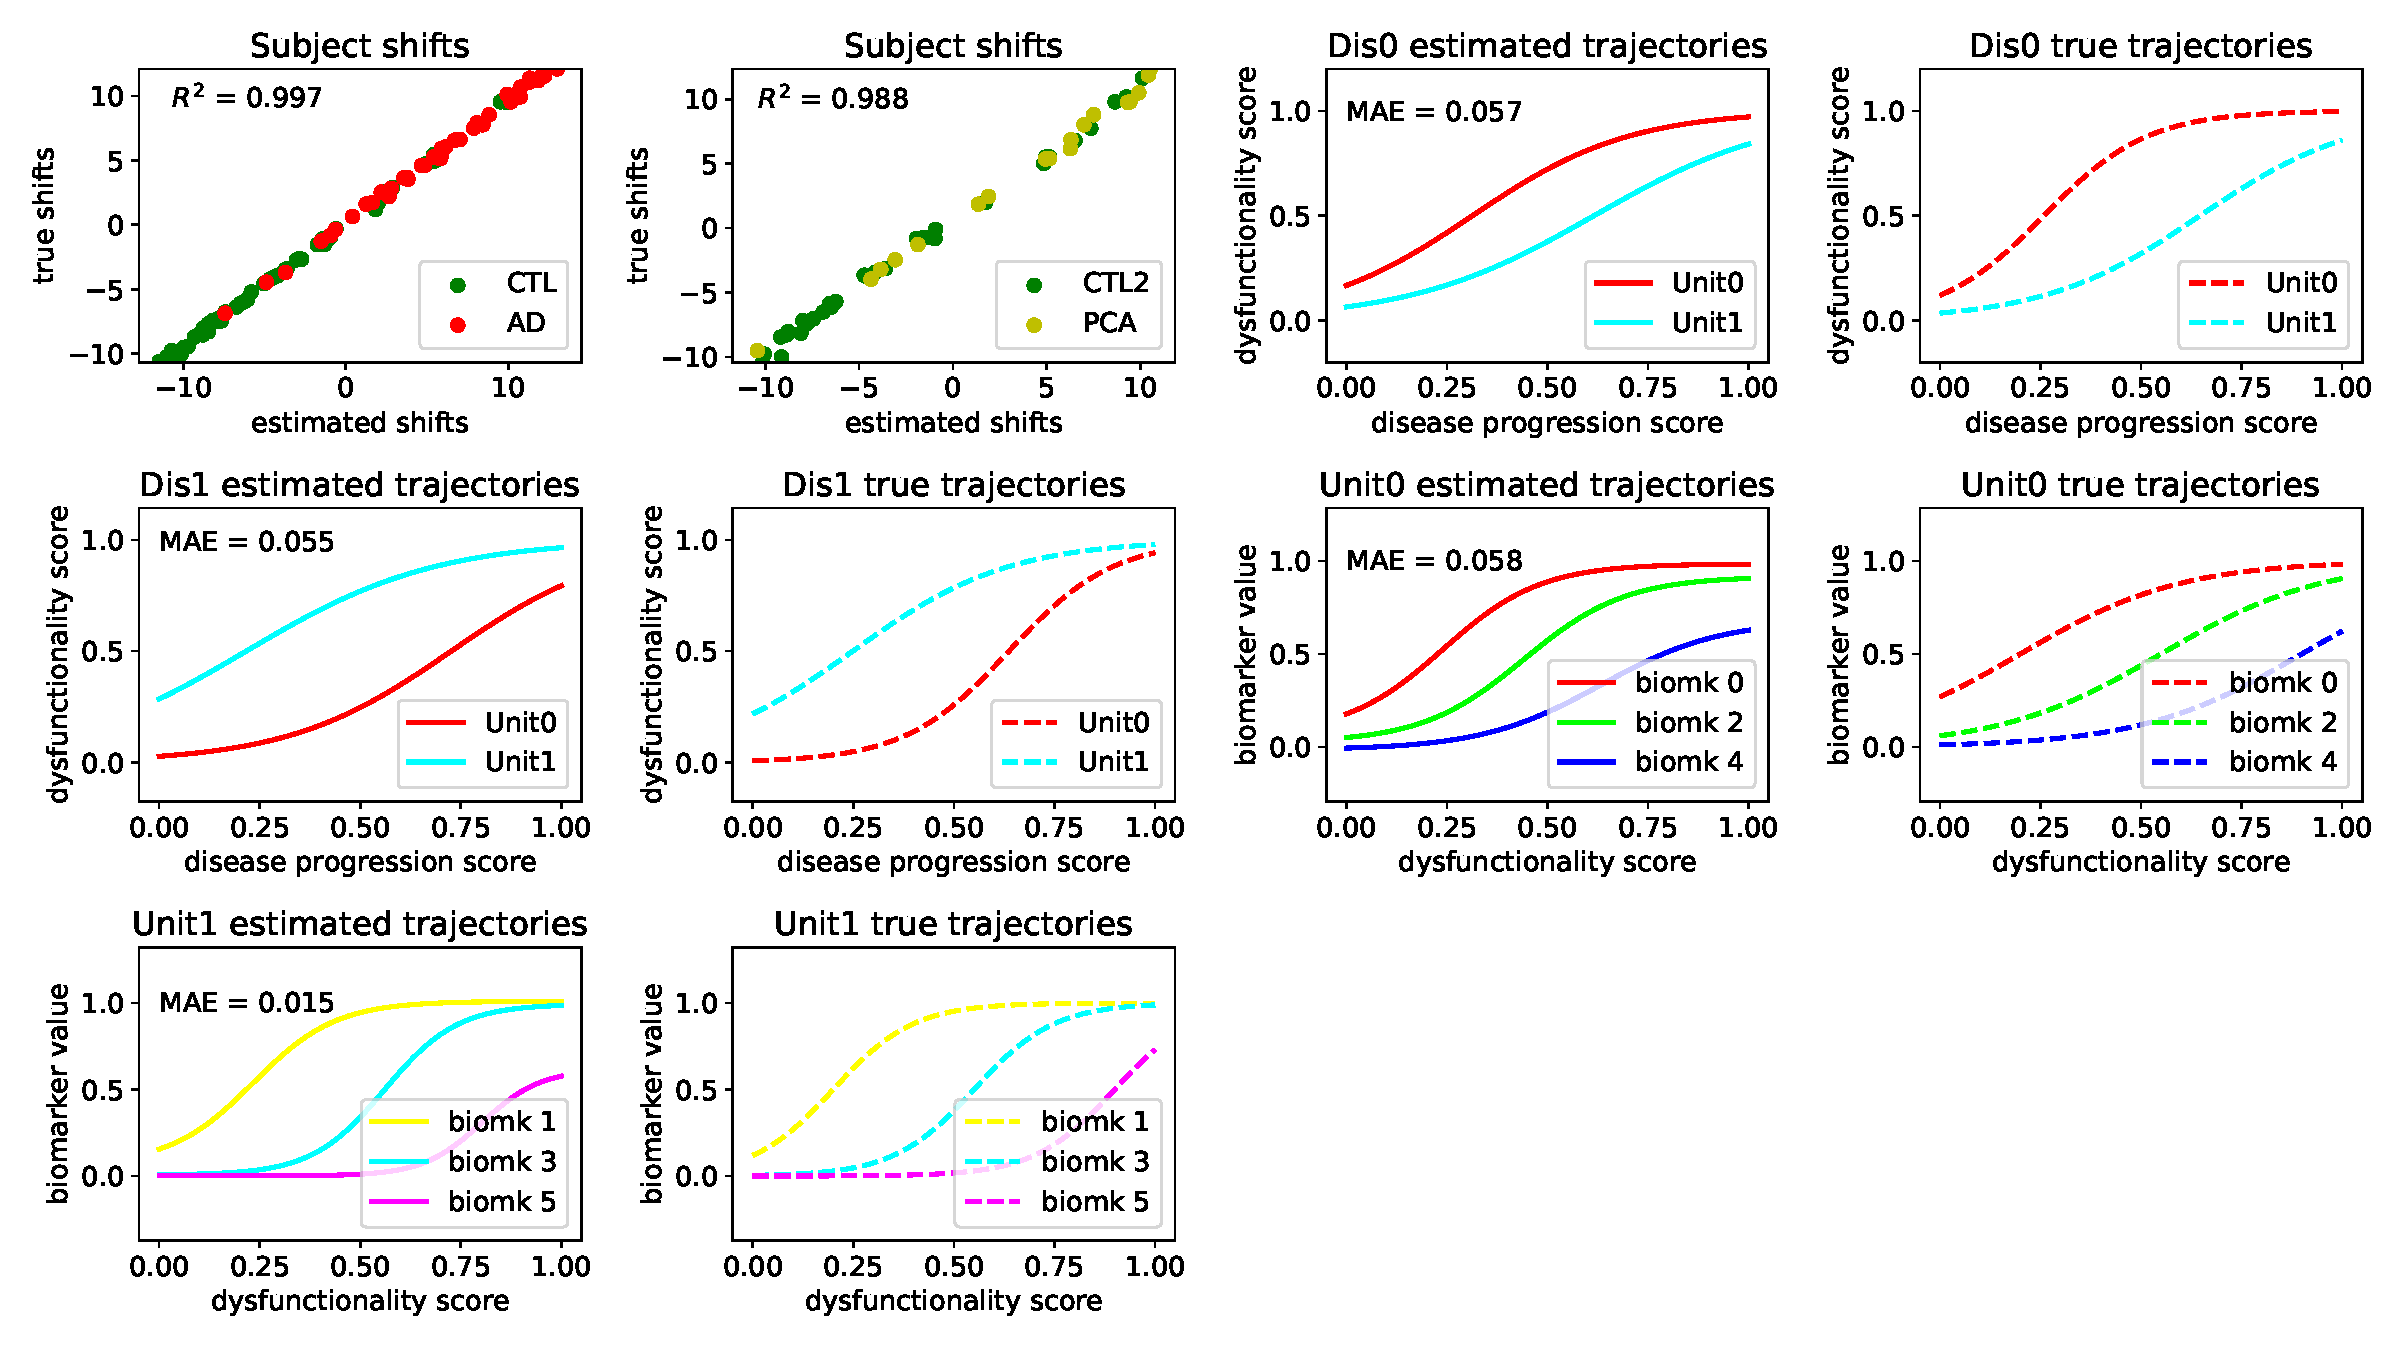
\includegraphics[width=\textwidth]{../resfiles/synth/synth1_JMD/compTrueParams101_synth1_JMD.pdf}
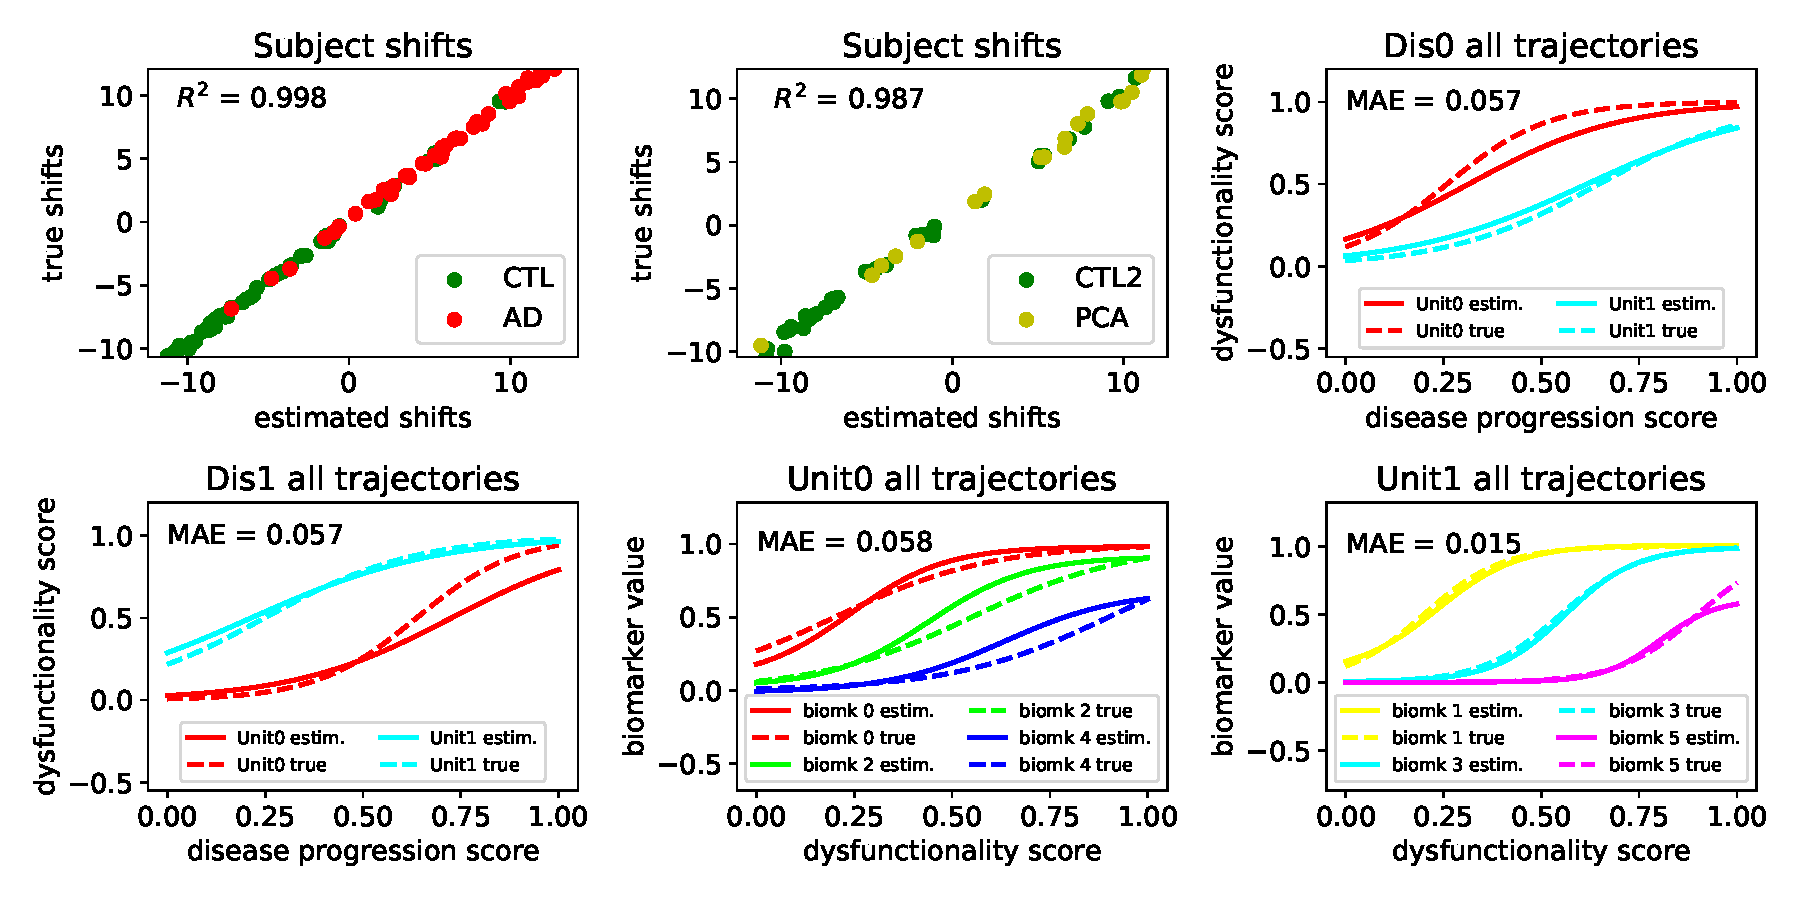
\includegraphics[width=0.4\textwidth]{../figures/compTrueParams105_synth1_JMD.pdf}
\caption[DKT Simulation Results - Comparison between true and DKT-estimated biomarker trajectories and subject time-shifts.]{Comparison between true and DKT-estimated subject time-shifts and biomarker trajectories.}
  \label{fig:dktSynthTrajCompTrue}
\end{figure}

\begin{figure}[H]
\centering
 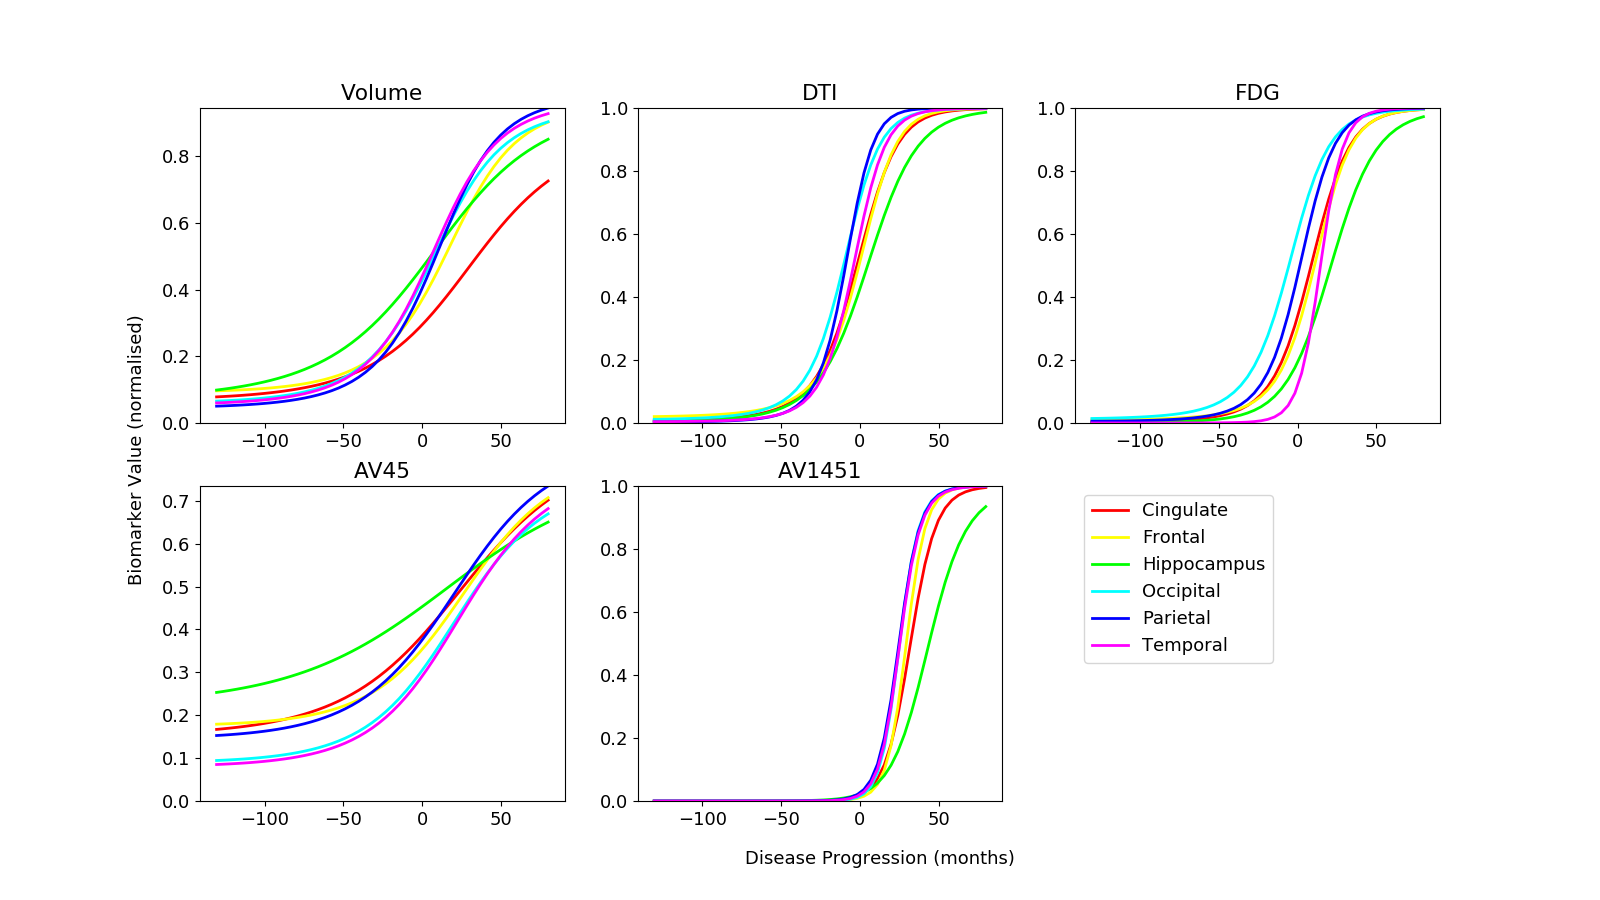
\includegraphics[width=0.4\textwidth, trim=0 20 0 0, clip]{../figures/trajDisSpaceOverlap_PCA_tad-drcTinyPen5_JMD.png}
 \caption{Estimated trajectories for the PCA cohort. The only data that were available were the MRI volumetric data. The dynamics of the other biomarkers has been inferred by the model using data from typical AD, and taking into account the different spatial distribution of pathology in PCA vs tAD. }
 \label{fig:PCAtrajByModality}
\end{figure}




\section*{Conclusion}






\end{multicols}
\hrule

\begin{multicols}{2}
 							%Use 3-column layout
\raggedcolumns	

\subsection*{References}

\large{
\begin{tabular}{l p{0.5cm} l}
 1. Fontejin et al., Neuroimg., 2012 & & 2. Young et al., Nat. Comms., 2018\\
 3. Villemagne et al., Lancet Neurol., 2013 & & 4. Marinescu et al., IPMI, 2017\\
\end{tabular}

\columnbreak

\subsection*{Weblinks}
\begin{itemize}
\item UCL Progression of Neurodegenerative Disease (POND): cmic.cs.ucl.ac.uk/pond/
\item UCL Centre for Medical Image Computing: www.ucl.ac.uk/cmic/
\end{itemize}
}


\vspace{1em}
% \hspace{2em}

\includegraphics[height=4.0cm]{epsrc_logo.jpg}
\hspace{0.5em}

\includegraphics[height=4.0cm]{pondLogo.png} 
\hspace{0.5em}

\includegraphics[height=4cm]{cdt_logo.png} 
\hspace{0.5em}

\includegraphics[height=4cm]{aruk_logo} 


\end{multicols}


\end{document}
